\documentclass[aps,prb,onecolumn,notitlepage,showpacs,floatfix,superscriptaddress]{revtex4-1}
\usepackage{dcolumn}
\usepackage{tabularx}
\usepackage{bm}
\usepackage{soul}
\usepackage{amsmath,amssymb,graphicx}
\usepackage[colorlinks=true,citecolor=blue,urlcolor=blue,linkcolor=blue]{hyperref}
\usepackage{environ}

\NewEnviron{eqnsplit}{%
\begin{equation}
\begin{split}
  \BODY
\end{split}
\end{equation}
}

\newcommand{\mrm}[1]{\mathrm{#1}}
\newcommand{\ang}{\mathrm{\AA}}

\bibliographystyle{apsrev4-1}

%%%%%%%%%%%%%%%%%%%%%%%%%%%%%%%%%%%%%%%%%%%%%%%%
\begin{document}
\title{Magnetism - Oscillations}

\author{Avinash Rustagi}
\email{arustag@ncsu.edu}
\affiliation{Department of Physics, North Carolina State University, Raleigh, NC 27695}
%
\date{\today}
%%%%%%%%%%%%%%%%%%%%%%%%%%%%%%%%%%%%%%%%%%%%%%%%

\maketitle

When dealing with magnetic fields in condensed matter physics, we encounter oscillations in resistivity i.e. Subhnikov de Haas oscillations and also in magnetization i.e. de Haas - van Alphen oscillations. These are crucial to characterize materials and thus a discussion is in order for them. In 1930's, Bohr and Leeuwen showed that magnetism cannot exist within the framework of classical mechanics. Considering the Hamiltonian for N-particles in 3D in presence of a magnetic field (included by minimal coupling)
\begin{equation}
H=\sum_{i=1}^{3N} \dfrac{(p_i-e A_i /c)^2}{2m} + V({\bm q}_1,{\bm q}_2,....{\bm q}_N)
\end{equation} 
The classical partition function can thus be evaluated 
\begin{equation}
Z_c = \int e^{-\beta H} \, d{\bm q}_1 d{\bm p}_1 d{\bm q}_2 d{\bm p}_2 ..... d{\bm q}_N d{\bm p}_N
\end{equation}
A shift of the momentum variables $p^\prime_i = p_i -e A_i/c$ removes the effect of the magnetic vector potential, thus any derivative of the partition function will not lead to magnetization i.e. magnetism. Hence we need quantum mechanics to study magnetism.

The Hamiltonian for a single electron in presence of magnetic field is
\begin{equation}
H=\dfrac{({\bm p}-e {\bm A}/c)^2}{2m} + V({\bm x}) + \mu_B {\bm \sigma}\cdot {\bm B} + \xi {\bm l}\cdot{\bm \sigma}
\end{equation}
where the Zeeman and Spin-Orbit interaction terms are included.
\begin{equation}
\xi = \dfrac{\hbar}{4 m^2 c^2} \dfrac{1}{r}\dfrac{dV}{dr} \qquad \text{and} \qquad \mu_B = \dfrac{\vert e \vert \hbar}{2 m c}
\end{equation}
For a constant field ${\bm B}$, the vector potential ${\bm A} = {\bm B} \times {\bm r}/2$,
\begin{equation}
\dfrac{({\bm p}-e {\bm A}/c)^2}{2m} = \dfrac{{\bm p}^2}{2m} - \dfrac{e}{2mc}({\bm r} \times {\bm p})\cdot {\bm B} + \dfrac{e^2}{8 m c^2} ({\bm B} \times {\bm r})^2
\end{equation}
Where if the field is in the z-direction
\begin{equation}
\dfrac{({\bm p}-e {\bm A}/c)^2}{2m} = \dfrac{{\bm p}^2}{2m} - \dfrac{e}{2mc}({\bm r} \times {\bm p})\cdot {\bm B} + \dfrac{e^2 B^2}{8 m c^2}  (x^2+y^2)
\end{equation}
Thus the complete Hamiltonian is
\begin{equation}
H= \dfrac{{\bm p}^2}{2m} + \mu_B \left(\dfrac{{\bm l}}{\hbar}+{\bm \sigma} \right)\cdot {\bm B} + \dfrac{e^2 B^2}{8 m c^2}  (x^2+y^2)+ V({\bm x}) + \xi {\bm l}\cdot{\bm \sigma}
\end{equation}
For a system with Z-electrons
\begin{equation}
H= \sum_{i=1}^Z \left[ \dfrac{{\bm p}_i ^2}{2m} + \mu_B \left(\dfrac{{\bm l}_i}{\hbar}+{\bm \sigma}_i \right)\cdot {\bm B} + \dfrac{e^2 B^2}{8 m c^2}  (x_i^2+y_i^2)+ V({\bm x}_i) + \xi {\bm l}_i \cdot{\bm \sigma}_i \right] + \dfrac{1}{2}\sum_{i \neq j}\dfrac{e^2}{\vert {\bm x}_i - {\bm x}_j \vert}
\end{equation}
We can simply compute the magnetization and susceptibility from the derivatives of the average energy in the T=0 limit.
\begin{equation}
M=-\dfrac{\partial \langle H \rangle}{\partial B} \qquad \chi = N_0 \dfrac{\partial M}{\partial B}
\end{equation}

\section{Diagmagnetism}
Consider the case of system with no spin-orbit interaction and no permanent magnetic moment. ($N_0$ Avagadro's Number for molar quantities)
\begin{equation}
\left\langle \dfrac{{l_z}_i}{\hbar}+{\sigma_z}_i \right\rangle =0
\end{equation}
Therefore
\begin{equation}
\begin{split}
M&=-\dfrac{\partial \langle H \rangle}{\partial B} = -\dfrac{e^2 B}{4 m c^2}  \sum_{i=1}^Z \langle x_i^2+y_i^2 \rangle\\
\chi_d &=N_0 \dfrac{\partial M}{\partial B} = -\dfrac{e^2 N_0}{4 m c^2}  \sum_{i=1}^Z \langle x_i^2+y_i^2 \rangle
\end{split}
\end{equation}
On symmetry grounds 
\begin{equation}
\sum_{i=1}^Z \langle x_i^2 \rangle = \sum_{i=1}^Z \langle y_i^2 \rangle = \dfrac{1}{3}\sum_{i=1}^Z \langle r_i^2 \rangle = \dfrac{1}{3} Z \langle r^2 \rangle
\end{equation}
\begin{equation}
\begin{split}
\chi_d &=N_0 \dfrac{\partial M}{\partial B} = -\dfrac{Z e^2 N_0}{6 m c^2}  \langle r^2 \rangle
\end{split}
\end{equation}
This is the atomic or diamagnetic susceptibility.

\section{de Haas - van Alphen Effect}
To understand this we need require the non-interacting Hamiltonian in presence of a magnetic field.
\begin{equation}
H=\sum_{i=1}^{N} \dfrac{({\bm p}-e{\bm A} /c)^2}{2m} + \sum_{i=1}^{N} \mu_B {\bm \sigma} \cdot {\bm B}
\end{equation}
where the first terms describes Landau levels, diamagnetism, and de Haas - van Alphen effect. The second term describes the Pauli paramagnetism.
\subsection{Landau Levels}
Considering the magnetic field in the z-direction, the vector potential can be chosen in the Landau gauge ${\bm A}=(0, Bx, 0)$. Thus the Schrodinger equation for the single electron Hamiltonian is
\begin{equation}
\left [ \dfrac{({\bm p}-e{\bm A} /c)^2}{2m} + \mu_B {\bm \sigma} \cdot {\bm B} \right] \psi = \varepsilon \psi
\end{equation}
where 
\begin{equation}
\begin{split}
&\varepsilon_{\sigma} (n,k_z)= \left(n+\dfrac{1}{2} \right) \hbar \omega_c + \dfrac{\hbar^2 k_z^2}{2m} + \sigma \mu_B B \quad n=0,1,2,...  \quad \sigma=\pm 1\\
&\psi_{n,k_y,k_z,\sigma}(x,y,z) \propto \exp\left( - k_y y + i k_z z\right) H_n \left( \dfrac{x-k_y l_B^2}{l_B} \right) \exp\left(-  \dfrac{(x-k_y l_B^2)^2}{2 l_B^2}\right)
\end{split}
\end{equation}
where 
\begin{equation}
\omega_c = \dfrac{\vert e \vert B}{m c} \quad  l_B =\sqrt{\dfrac{\hbar}{m \omega_c}}
\end{equation}
The system is clearly periodic in y- and z-directions and thus $k_y$ and $k_z$ are integer multiples of $2\pi/L_y$ and $2\pi/L_z$. However, we can see from the wavefunction that we have a shifted Harmonic oscillator with the center as $k_y l_B^2$. The center needs to lie within the sample
\begin{equation}
-\dfrac{L_x	}{2} \leq k_y l_B^2 \leq \dfrac{L_x}{2}
\end{equation}
This implies that 
\begin{equation}
-\dfrac{e B L_x}{2 \hbar c} \leq k_y  \leq \dfrac{|e| B L_x}{2 \hbar c}
\end{equation}
Thus the degeneracy of each LL is
\begin{equation}
\dfrac{k_y^{max}-k_y^{min}}{2\pi/L_y} = \dfrac{|e| B L_x L_y}{2 \pi \hbar c}
\end{equation}
Let us define $N_\sigma (\varepsilon)$ as the number of states with energy $\varepsilon_\sigma \leq \varepsilon$. To obtain this quantity, we need to multiply the number of possible values of $k_z$ by the LL degeneracy for given values of $n$ and $\sigma$ and energy $\varepsilon \leq \varepsilon_\sigma (n,k_z)$. 
\begin{equation}
k_z^{max/min} = \pm \dfrac{\sqrt{2m}}{\hbar} \sqrt{\varepsilon - \hbar \omega_c \left(n+\dfrac{1}{2}\right)-\sigma \mu_B B}
\end{equation}
Therefore the number of states with energy $\varepsilon \leq \varepsilon_n$ are
\begin{equation}
\dfrac{k_z^{max}-k_z^{min}}{2\pi/L_z} =  \dfrac{L_z \sqrt{2m}}{\pi\hbar} \sqrt{\varepsilon - \hbar \omega_c \left(n+\dfrac{1}{2}\right)-\sigma \mu_B B}
\end{equation}
Therefore all possible state with energy $\varepsilon$ is
\begin{equation}
N_\sigma (\varepsilon) = \dfrac{|e| B \sqrt{2m} L_x L_y L_z }{2 \pi^2 \hbar^2 c} \sum_{n=0}^{n_{max}} \sqrt{\varepsilon - \hbar \omega_c \left(n+\dfrac{1}{2}\right)-\sigma \mu_B B}
\end{equation}
where $n_{max}$ is the maximum allowed $n$ for which the square root is real.

\subsection{Free Energy}
For a given Hamiltonian of the kind
\begin{equation}
H=\sum_\alpha \left(\varepsilon_\alpha - \mu \right) n_\alpha
\end{equation}
The thermodynamic potential in the grand canonical ensemble is
\begin{equation}
\Omega = -k_B T \log Z
\end{equation}
where the partition function is given by
\begin{equation}
\begin{split}
Z &= \sum_{\{n_\alpha = 0,1 \}} \exp\left[-\beta H \right] = \sum_{\{n_\alpha = 0,1 \}} \exp\left[-\beta \sum_\alpha \left(\varepsilon_\alpha - \mu \right) n_\alpha \right] \\
&= \prod_{\alpha}\sum_{\{n_\alpha = 0,1 \}} \exp\left[-\beta \left(\varepsilon_\alpha - \mu \right) n_\alpha \right] \\
&= \prod_{\alpha} \left[1+ e^{-\beta(\varepsilon_\alpha - \mu)} \right]
\end{split}
\end{equation}
Therefore 
\begin{equation}
\Omega = -k_B T \log Z = -k_B T \sum_{\alpha}\log \left[1+ e^{-\beta(\varepsilon_\alpha - \mu)} \right]
\end{equation}
The Helmholtz Free Energy is thus
\begin{equation}
\begin{split}
F&=\Omega + \mu N = N \mu -k_B T \log Z = N\mu -k_B T \sum_{\alpha} \log\left[1+ e^{-\beta(\varepsilon_\alpha - \mu)} \right] \\
&= N\mu -k_B T \sum_{\sigma=\pm 1} \int d\varepsilon \log\left[1+ e^{-\beta(\varepsilon - \mu)} \right] D_\sigma (\varepsilon)
\end{split}
\end{equation}
where $D_\sigma (\varepsilon)$ is the density of states with energy $\varepsilon$ which can be written as
\begin{equation}
D_\sigma (\varepsilon) = \dfrac{d N_\sigma (\varepsilon)}{d\varepsilon}
\end{equation}
where $N_\sigma (\varepsilon)$ is the number of states upto energy $\varepsilon$.
\begin{equation}
\begin{split}
F &= N\mu -k_B T \sum_{\sigma=\pm 1} \int d\varepsilon \log\left[1+ e^{-\beta(\varepsilon - \mu)} \right]  \dfrac{d N_\sigma (\varepsilon)}{d\varepsilon} \\
&= N\mu - \sum_{\sigma=\pm 1} \int d\varepsilon f(\varepsilon) N_\sigma (\varepsilon)
\end{split}
\end{equation}
where 
\begin{equation}
f(\varepsilon) = \dfrac{1}{1+e^{\beta(\varepsilon - \mu)}}
\end{equation}
Therefore
\begin{equation}
\begin{split}
F &= N\mu - \dfrac{|e| B \sqrt{2m} L_x L_y L_z }{2 \pi^2 \hbar^2 c}  \sum_{\sigma=\pm 1} \int d\varepsilon \dfrac{1}{1+e^{\beta(\varepsilon - \mu)}} \sum_{n=0}^{n_{max}} \sqrt{\varepsilon - \hbar \omega_c \left(n+\dfrac{1}{2}\right)-\sigma \mu_B B}
\end{split}
\end{equation}
Defining dimensionless variables
\begin{equation}
\mu_B = \dfrac{|e| \hbar	}{2 m c} \quad E_0 = \dfrac{\mu}{2 \mu_B B} \quad E = \dfrac{\varepsilon}{2 \mu_B B} \quad \Theta = \dfrac{k_B T}{2 \mu_B B} \quad \Omega = L_x L_y L_z
\end{equation}
In terms of which
\begin{equation}
\begin{split}
F &= N\mu - \dfrac{|e| B \sqrt{2m} \Omega (2 \mu_B B)^{3/2}}{2 \pi^2 \hbar^2 c}  \sum_{\sigma=\pm 1} \int dE \dfrac{1}{1+e^{(E-E_0)/\Theta}} \sum_{n=0}^{n_{max}} \sqrt{E - n - \dfrac{1}{2}-\dfrac{\sigma}{2}} \\
&= N\mu - \dfrac{ 4 m^{3/2} \Omega (\mu_B B)^{5/2}}{ \pi^2 \hbar^3 }  \sum_{\sigma=\pm 1} \int dE \dfrac{1}{1+e^{(E-E_0)/\Theta}} \sum_{n=0}^{n_{max}} \sqrt{E - n - \dfrac{1}{2}-\dfrac{\sigma}{2}} \\
&= N\mu - \dfrac{ 4 m^{3/2} \Omega (\mu_B B)^{5/2}}{ \pi^2 \hbar^3 }  \sum_{\sigma=\pm 1} \int dE f(E) \sum_{n=0}^{n_{max}} \dfrac{2}{3}\dfrac{d}{dE} \left(E - n - \dfrac{1}{2}-\dfrac{\sigma}{2}\right)^{3/2} \\
&= N\mu + \dfrac{ 8 m^{3/2} \Omega (\mu_B B)^{5/2}}{ 3 \pi^2 \hbar^3 }  \sum_{\sigma=\pm 1} \int_{-\infty}^\infty dE f'(E) \sum_{n=0}^{n_{max}}  \left(E - n - \dfrac{1}{2}-\dfrac{\sigma}{2}\right)^{3/2} \\
&= N\mu + \alpha \sum_{\sigma=\pm 1} \int_{-\infty}^\infty dE f'(E) \sum_{n=0}^{n_{max}}  \left(E - n - \dfrac{1}{2}-\dfrac{\sigma}{2}\right)^{3/2} \\
&= N\mu + \alpha \int_{-\infty}^\infty dE \left[ f'(E + 1/2) + f'(E-1/2) \right] \sum_{n=0}^{n_{max}}  \left(E - n - \dfrac{1}{2}\right)^{3/2} \\
\end{split}
\end{equation}
To evaluate the above, we use the identity
\begin{equation}
\sum_{n=0}^{n_{max}}  \left(E - n - \dfrac{1}{2}\right)^{3/2}  = \sum_{l=-\infty}^\infty (-1)^l \int_0^E dx \, (E-x)^{3/2} e^{2\pi i l x}
\end{equation}
\noindent\makebox[\linewidth]{\rule{\textwidth}{0.4pt}}
\textbf{Proof:} Poisson Formula \\
A periodic function with period $T$ can be Fourier expanded.
\begin{equation}
x(t) = \sum_{l=-\infty}^\infty x(l) e^{2\pi i l t/T}
\end{equation}
The Fourier coefficients of the expansion are
\begin{equation}
x(l) = \dfrac{1}{T} \int_{-T/2}^{T/2} dt \, x(t) e^{-2\pi i l t/T}
\end{equation}
Considering the periodic function to be a Dirac comb
\begin{equation}
x(t) = \sum_{n=-\infty}^{\infty} \delta(t-n T)
\end{equation}
the corresponding coefficients are
\begin{equation}
\begin{split}
x(l) &= \dfrac{1}{T} \int_{-T/2}^{T/2} dt \, \sum_{n=-\infty}^{\infty} \delta(t-nT) e^{-2\pi i l t/T} \\
&= \dfrac{1}{T} \int_{-T/2}^{T/2} dt \, \delta(t) e^{-2\pi i l t/T} \\
&=\dfrac{1}{T}
\end{split}
\end{equation}
Therefore
\begin{equation}
x(t) = \sum_{l=-\infty}^\infty x(l) e^{2\pi i l t/T} \Rightarrow \sum_{n=-\infty}^{\infty} \delta(t-nT) = \dfrac{1}{T} \sum_{l=-\infty}^\infty  e^{2\pi i l t/T}
\end{equation}
Choosing the period to be $T=1$,
\begin{equation}
\sum_{n=-\infty}^{\infty} \delta(t-n) = \sum_{l=-\infty}^\infty  e^{2\pi i l t}
\end{equation}
Thus for a Dirac comb of the form $\sum_{n=-\infty}^{\infty} \delta(t-n -1/2) $
\begin{equation}
\sum_{n=-\infty}^{\infty} \delta(t-n-1/2) = \sum_{l=-\infty}^\infty  e^{2\pi i l (t-1/2)}
\end{equation}
If we now multiply the Poisson formula by a function and integrate as shown
\begin{equation}
\begin{split}
\int_0^\infty dt \, f(t) \sum_{n=-\infty}^{\infty} \delta(t-n-1/2) &= \int_0^\infty dt \, f(t) \sum_{l=-\infty}^\infty  e^{2\pi i l (t-1/2)} \\
\Rightarrow \quad  \sum_{n=0}^{\infty} f(n+1/2) & = \int_0^\infty dt \, f(t) \sum_{l=-\infty}^\infty  e^{2\pi i l (t-1/2)} \\
&= \sum_{l=-\infty}^\infty  \int_0^\infty dt \, f(t)  e^{2\pi i l t} e^{i\pi l} \\
&= \sum_{l=-\infty}^\infty  \int_0^\infty dt \, f(t)  e^{2\pi i l t} (-1)^l \\
\end{split}
\end{equation}
Now to consider a finite sum, we can construct a composite function $f(t)$ which is non-zero for $n<n_{max}$ and $0$ for $n>n_{max}$. For $n=n_{max}$, $t=E$,
\begin{equation}
\begin{split}
\sum_{n=0}^{n_{max}} f(n+1/2) &= \sum_{l=-\infty}^\infty  \int_0^E dt \, f(t)  e^{2\pi i l t} (-1)^l \\
\end{split}
\end{equation}
If $f(t)=(E-t)^{3/2}$,
\begin{equation}
\begin{split}
\sum_{n=0}^{n_{max}} (E-n-1/2)^{3/2} &= \sum_{l=-\infty}^\infty  (-1)^l  \int_0^E dt \, (E-t)^{3/2}  e^{2\pi i l t} \\
\end{split}
\end{equation}
\noindent\makebox[\linewidth]{\rule{\textwidth}{0.4pt}}
To continue with the evaluation of the free energy
\begin{equation}
\begin{split}
\sum_{n=0}^{n_{max}}  \left(E - n - \dfrac{1}{2}\right)^{3/2}  &= \sum_{l=-\infty}^\infty (-1)^l \int_0^E dx \, (E-x)^{3/2} e^{2\pi i l x} \\
&= \int_0^E dx \, (E-x)^{3/2}  + \sum_{l=1}^\infty \int_0^E dx \, (E-x)^{3/2} \left[ (-1)^l e^{2\pi i l x} + (-1)^{-l} e^{-2\pi i l x} \right] \\
&= \int_0^E dx \, (E-x)^{3/2}  + 2 \sum_{l=1}^\infty \int_0^E dx \, (E-x)^{3/2} (-1)^l   \text{Re}\left[ e^{2\pi i l x} \right] \\
&= \dfrac{2}{5} E^{5/2} + 2 \sum_{l=1}^\infty \int_0^E dx \, (E-x)^{3/2} (-1)^l   \text{Re}\left[ e^{2\pi i l x} \right] \\
&= \dfrac{2}{5} E^{5/2} + 2 \sum_{l=1}^\infty  (-1)^l   \text{Re}\left[ \int_0^E dx \, (E-x)^{3/2} e^{2\pi i l x} \right] \\
&= \dfrac{2}{5} E^{5/2} + 2 \sum_{l=1}^\infty  (-1)^l   \text{Re}\left[ \int_0^E dx \, (E-x)^{3/2} \dfrac{d}{dx}\dfrac{e^{2\pi i l x}}{2\pi i l} \right]\\
&= \dfrac{2}{5} E^{5/2} + 2 \sum_{l=1}^\infty  (-1)^l   \text{Re}\left[(E-x)^{3/2}\dfrac{e^{2\pi i l x}}{2\pi i l} \bigg\vert_0^E- \dfrac{3}{2} \int_0^E dx \, (E-x)^{1/2} \dfrac{e^{2\pi i l x}}{2\pi i l} \right] \\
&= \dfrac{2}{5} E^{5/2} + 2 \sum_{l=1}^\infty  (-1)^l   \text{Re}\left[-\dfrac{E^{3/2}}{2\pi i l} - \dfrac{3}{2} \dfrac{1}{2\pi i l}\int_0^E dx \, (E-x)^{1/2} \dfrac{d}{dx}\dfrac{e^{2\pi i l x}}{2\pi i l} \right] \\
\end{split}
\end{equation}
the first term after the integration by parts is purely imaginary and thus can be dropped,
\begin{equation}
\begin{split}
\sum_{n=0}^{n_{max}}  \left(E - n - \dfrac{1}{2}\right)^{3/2}  &= \dfrac{2}{5} E^{5/2} + 2 \sum_{l=1}^\infty  (-1)^l   \text{Re}\left[ - \dfrac{3}{2} \dfrac{1}{2\pi i l}\int_0^E dx \, (E-x)^{1/2} \dfrac{d}{dx}\dfrac{e^{2\pi i l x}}{2\pi i l} \right] \\
&= \dfrac{2}{5} E^{5/2} + 2 \sum_{l=1}^\infty  (-1)^l   \text{Re}\left[  \dfrac{3}{2} \dfrac{E^{1/2}}{(2\pi i l)^2}  + \dfrac{3}{4} \dfrac{1}{2\pi i l}\int_0^E dx \, (E-x)^{-1/2} \dfrac{e^{2\pi i l x}}{2\pi i l} \right] \\
&= \dfrac{2}{5} E^{5/2} + 2 \sum_{l=1}^\infty  (-1)^l   \text{Re}\left[  - \dfrac{3 E^{1/2}}{8\pi^2 l^2}  - \dfrac{3}{16 \pi^2 l^2} \int_0^E dx \, (E-x)^{-1/2} e^{2\pi i l x} \right] \\
&= \dfrac{2}{5} E^{5/2} - \sum_{l=1}^\infty  (-1)^l \dfrac{3 E^{1/2}}{4\pi^2 l^2} -  \sum_{l=1}^\infty  (-1)^l \dfrac{3}{8 \pi^2 l^2}   \text{Re}\left[  \int_0^E dx \, (E-x)^{-1/2} e^{2\pi i l x} \right] \\
\end{split}
\end{equation}
Using
\begin{equation}
\sum_{l=1}^\infty \dfrac{(-1)^l}{l^2} = -\dfrac{\pi^2}{12}
\end{equation}
\begin{equation}
\begin{split}
\sum_{n=0}^{n_{max}}  \left(E - n - \dfrac{1}{2}\right)^{3/2}  &= \dfrac{2}{5} E^{5/2}  + \dfrac{E^{1/2}}{16} -  \sum_{l=1}^\infty  (-1)^l \dfrac{3}{8 \pi^2 l^2}   \text{Re}\left[  \int_0^E dx \, (E-x)^{-1/2} e^{2\pi i l x} \right] \\
\end{split}
\end{equation}
substituting $x=E-u^2$,
\begin{equation}
\begin{split}
\sum_{n=0}^{n_{max}}  \left(E - n - \dfrac{1}{2}\right)^{3/2}  &= \dfrac{2}{5} E^{5/2}  + \dfrac{E^{1/2}}{16} -  \sum_{l=1}^\infty  (-1)^l \dfrac{3}{4 \pi^2 l^2}   \text{Re}\left[  \int_0^{\sqrt{E}} du \,  e^{2\pi i l (E-u^2)} \right] \\
\end{split}
\end{equation}
This can now be substituted in the expression for the free energy
\begin{equation}
\begin{split}
F &= N\mu + \alpha \int_{-\infty}^\infty dE \left[ f'(E + 1/2) + f'(E-1/2) \right]\left( \dfrac{2}{5} E^{5/2}  + \dfrac{E^{1/2}}{16} -  \sum_{l=1}^\infty  (-1)^l \dfrac{3}{4 \pi^2 l^2}   \text{Re}\left[  \int_0^{\sqrt{E}} du \,  e^{2\pi i l (E-u^2)} \right]\right) \\
&= F_o + F_{osc}
\end{split}
\end{equation}
where $F_o$ contains the non-oscillatory terms whereas $F_{osc}$ has the oscillatory terms.
\begin{equation}
F_{osc} = - \alpha \int_{-\infty}^\infty dE \left[ f'(E + 1/2) + f'(E-1/2) \right]\left(\sum_{l=1}^\infty  (-1)^l \dfrac{3}{4 \pi^2 l^2}   \text{Re}\left[  e^{2\pi i l E} \int_0^{\sqrt{E}} du \,  e^{-2\pi i l u^2} \right]\right) \\
\end{equation}
The $u$-integral is an error function. Since the Fermi function derivative is peaked about $E_0$ i.e. dimensionless chemical potential, we can replace the upper limit of $u$-integral by $\infty$
\begin{equation}
\begin{split}
F_{osc} &= - \alpha \int_{-\infty}^\infty dE \left[ f'(E + 1/2) + f'(E-1/2) \right]\left(\sum_{l=1}^\infty  (-1)^l \dfrac{3}{4 \pi^2 l^2}   \text{Re}\left[  e^{2\pi i l E} \int_0^{\infty} du \,  e^{-2\pi i l u^2} \right]\right) \\
 &= - \alpha \int_{-\infty}^\infty dE  f'(E )  \left(\sum_{l=1}^\infty  (-1)^l \dfrac{3}{4 \pi^2 l^2}   \text{Re}\left[ ( e^{2\pi i l (E+1/2)} + e^{2\pi i l (E-1/2)}) \dfrac{e^{-i\pi/4}}{2\sqrt{2l}} \right]\right) \\
 &= - \alpha \int_{-\infty}^\infty dE  f'(E )  \left(\sum_{l=1}^\infty  (-1)^l \dfrac{3}{4 \pi^2 l^2}   \text{Re}\left[ 2 \cos(\pi l) e^{2\pi i l E}\dfrac{e^{-i\pi/4}}{2\sqrt{2l}} \right]\right) \\
 &= - \alpha  \sum_{l=1}^\infty  (-1)^l \dfrac{3}{4\sqrt{2} \pi^2 l^{5/2}}   \cos(\pi l) \text{Re}\left[  \int_{-\infty}^\infty dE  f'(E ) e^{2\pi i l E -i\pi/4} \right] \\
\end{split}
\end{equation}
Thus we need to evaluate the integral
\begin{equation}
\begin{split}
\int_{-\infty}^\infty dE  f'(E ) e^{2\pi i l E -i\pi /4} &= -2\pi i l \int_{-\infty}^\infty dE  f(E ) e^{2\pi i l E -i\pi /4} \quad \text{ignoring the surface term in integration by parts} \\
 &= -2\pi i l \int_{-\infty}^\infty dE  \dfrac{1}{1+e^{(E-E_0)/\Theta}} e^{2\pi i l E -i\pi /4} \\
 &= -2\pi i l \Theta \int_{-\infty}^\infty dy  \dfrac{1}{1+e^{y}} e^{2\pi i l (\Theta y + E_0) -i\pi /4} \\
 &= -2\pi i l \Theta e^{2\pi i l  E_0 -i\pi /4} \int_{-\infty}^\infty dy  \dfrac{1}{1+e^{y}} e^{2\pi i l \Theta y } \\
 \end{split}
\end{equation}
\begin{figure}[ht]
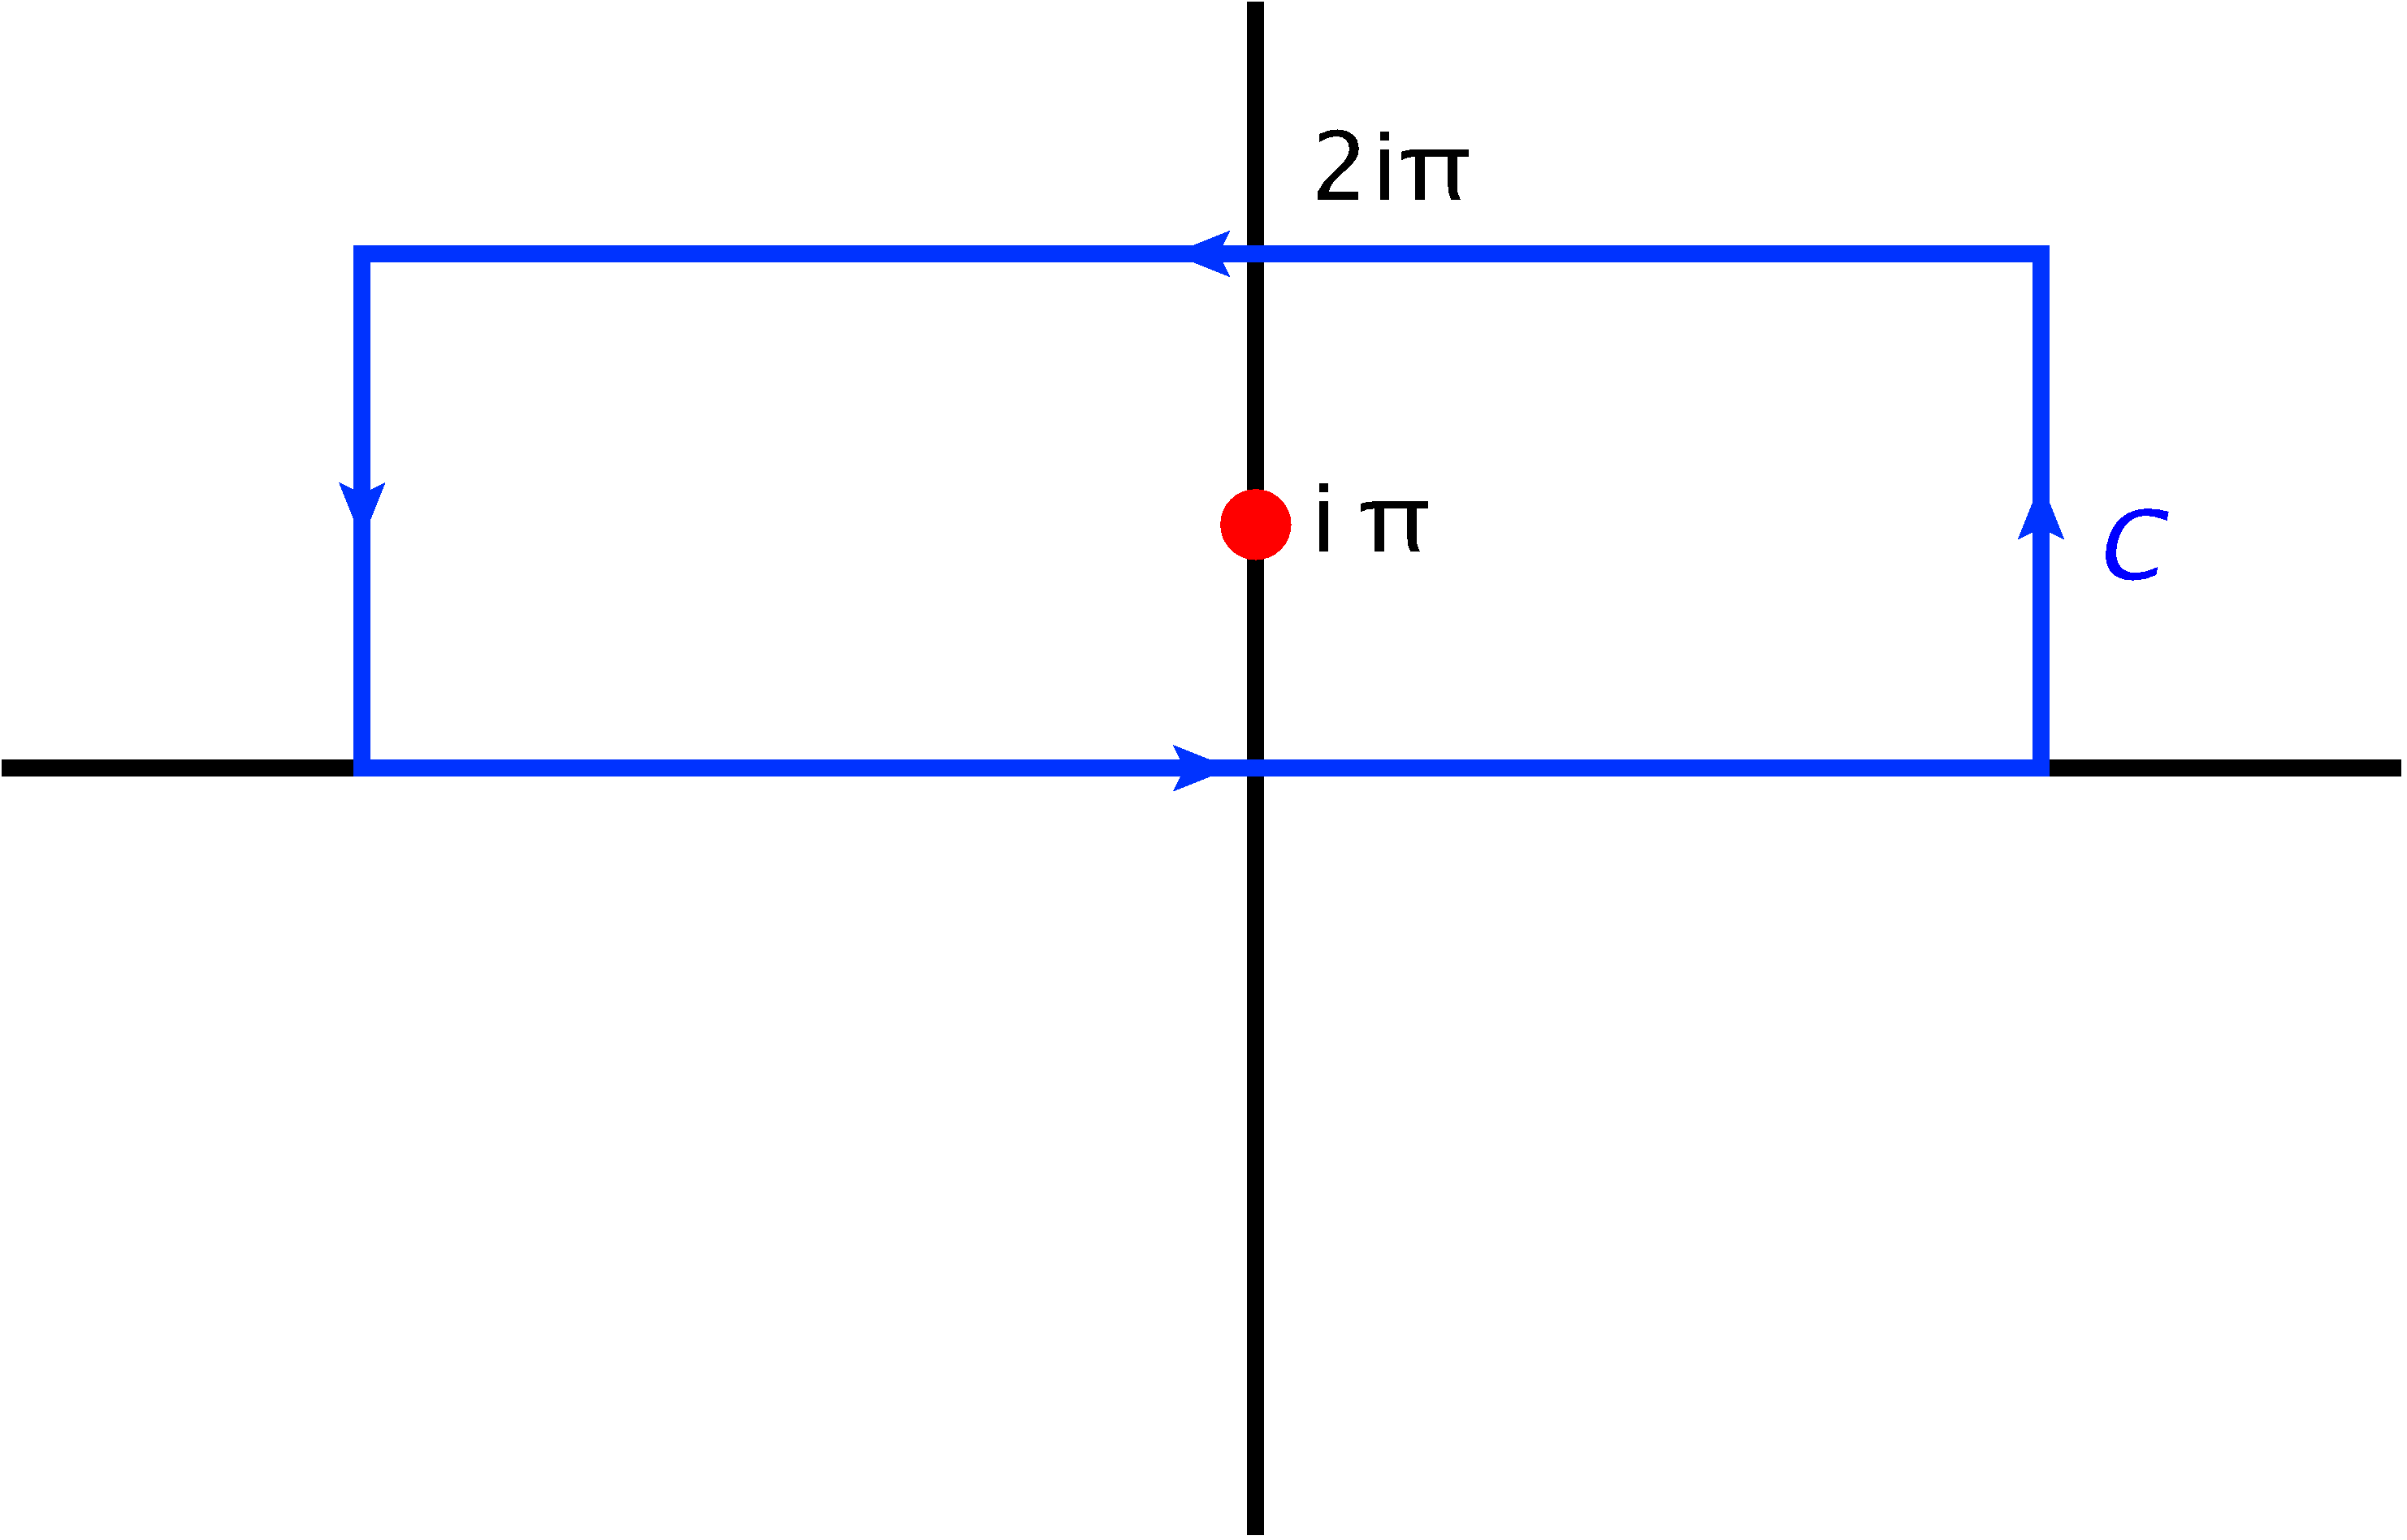
\includegraphics[scale=0.06]{contour.png} 
\end{figure}
To solve this consider the contour integral
\begin{equation}
\oint_C dz  \dfrac{1}{1+e^{z}} e^{2\pi i l \Theta z } \\
\end{equation}
where the function has poles at $z=\pm (2n+1)i \pi$. Choosing the contour of the form shown which includes a pole at $z=+i\pi$. Therefore
\begin{equation}
\begin{split}
&\oint_C dz  \dfrac{1}{1+e^{z}} e^{2\pi i l \Theta z } = 2\pi i \text{Res} \vert_{i\pi} \\
&\int_{-\infty}^\infty dy  \dfrac{1}{1+e^{y}} e^{2\pi i l \Theta y } + \int_{\infty}^{-\infty} dy  \dfrac{1}{1+e^{y+2\pi i}} e^{2\pi i l \Theta (y+2 \pi i) }  = 2\pi i  e^{-2\pi^2 l \Theta }\\
&\int_{-\infty}^\infty dy  \dfrac{1}{1+e^{y}} e^{2\pi i l \Theta y } (1-e^{-4\pi^2 l \Theta })  = 2\pi i  e^{-2\pi^2 l \Theta } \\
&\int_{-\infty}^\infty dy  \dfrac{1}{1+e^{y}} e^{2\pi i l \Theta y }   = 2\pi i  \dfrac{e^{-2\pi^2 l \Theta }}{(1-e^{-4\pi^2 l \Theta })} = \dfrac{\pi i}{\sinh(2\pi^2 l \Theta)}
\end{split}
\end{equation}
Therefore
\begin{equation}
\begin{split}
\int_{-\infty}^\infty dE  f'(E ) e^{2\pi i l E -i\pi /4} &= -2\pi i l \Theta e^{2\pi i l  E_0 -i\pi /4} \int_{-\infty}^\infty dy  \dfrac{1}{1+e^{y}} e^{2\pi i l \Theta y } \\
&=  e^{2\pi i l  E_0 -i\pi /4} \dfrac{2\pi^2  l \Theta}{\sinh(2\pi^2 l \Theta)} \\
 \end{split}
\end{equation}
and thus the free energy
\begin{equation}
\begin{split}
F_{osc} &= - \alpha  \sum_{l=1}^\infty  (-1)^l \dfrac{3}{4\sqrt{2} \pi^2 l^{5/2}}   \cos(\pi l) \text{Re}\left[  \int_{-\infty}^\infty dE  f'(E ) e^{2\pi i l E -i\pi/4} \right] \\
 &= - \alpha  \sum_{l=1}^\infty  (-1)^l \dfrac{3}{4\sqrt{2} \pi^2 l^{5/2}}   \cos(\pi l) \text{Re}\left[ e^{2\pi i l  E_0 -i\pi /4} \dfrac{2\pi^2  l \Theta}{\sinh(2\pi^2 l \Theta)}   \right] \\
  &= - \alpha  \sum_{l=1}^\infty  (-1)^l \dfrac{3}{4\sqrt{2} \pi^2 l^{5/2}}   \dfrac{2\pi^2  l \Theta}{\sinh(2\pi^2 l \Theta)}   \cos(\pi l) \cos(2\pi l  E_0 -\pi /4) \\
 &= - \alpha  \sum_{l=1}^\infty  (-1)^l \dfrac{3}{2\sqrt{2}  l^{3/2}} \Theta \cos(\pi l)  \dfrac{\cos(2\pi l  E_0 -\pi /4)}{\sinh(2\pi^2 l \Theta)}     \\
  &= - \alpha  \sum_{l=1}^\infty  (-1)^l \dfrac{3}{2\sqrt{2}  l^{3/2}} \dfrac{k_B T}{2\mu_B B} \cos(\pi l)  \dfrac{\cos\left(  \dfrac{\pi l\mu}{\mu_B B} -\dfrac{\pi} {4}\right)}{\sinh\left( \dfrac{\pi^2 l k_B T}{\mu_B B} \right)}     \\
\end{split}
\end{equation}
Given that the free energy has an oscillatory dependence on the magnetic field, the resultant measurements of magnetization also has oscillatory dependence.
\end{document}